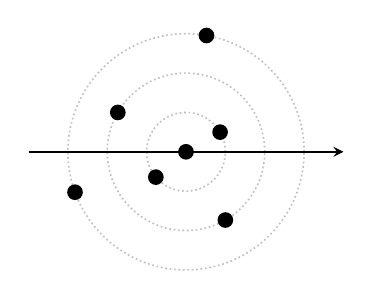
\begin{tikzpicture}[semithick, font = \scriptsize, label distance = 0pt, every node/.style = { inner sep = 2pt, circle, fill }]
  \draw [densely dotted, draw = lightgray] (0, 0) circle (0.5);
  \draw [densely dotted, draw = lightgray] (0, 0) circle (1);
  \draw [densely dotted, draw = lightgray] (0, 0) circle (1.5);
  \draw [-stealth, draw = black] (-2, 0) -- (2, 0);

  \node (medication) at (0, 0) {};
  \node (antipyretic) at (30:0.5) {};
  \node (vaccine) at (220:0.5) {};
  \node (aspirin) at (150:1) {};
  \node (a) at (300:1) {};
  \node (b) at (200:1.5) {};
  \node (c) at (80:1.5) {};
\end{tikzpicture}
